\documentclass[12pt]{article}

\usepackage[margin=1in]{geometry}
\usepackage{amsmath,amssymb}
\usepackage{graphicx}
\usepackage{booktabs}
\usepackage{caption}
\usepackage{mathptmx} % Times-like text/math, common in IS journal templates
\usepackage[hyphens]{url}
\usepackage{natbib}
\usepackage{hyperref}
\usepackage{setspace}
\usepackage{authblk}

\hypersetup{colorlinks=true, linkcolor=black, citecolor=black, urlcolor=black}

\title{\textbf{Faster but More Concentrated: A Difference-in-Differences\\
Study of AI Coding-Tool Adoption and Code Review Dynamics on GitHub}}

\author[1]{[Author Name]}
\date{}

\begin{document}

\maketitle

\begin{abstract}
\noindent Generative-AI coding assistants (e.g., GitHub Copilot, Cursor,
Claude Code) are now embedded in everyday software development, but their
effect on the human coordination work that surrounds code---specifically,
peer code review---is not well understood. We estimate the causal effect
of a repository's own adoption of an AI coding tool on its code-review
process using a staggered-adoption difference-in-differences design,
implemented with the imputation estimator of
\citet{borusyak2024revisiting}, on a matched sample of 1,771
treated/control GitHub repository pairs (20,188 repository-month
observations). Grounding three hypotheses in a verification-cost account
of human--AI collaboration, we examine whether adoption changes review
dependence (H1, primary), latency (H2), and iteration (H3), alongside
review intensity as a benchmark. The estimates show no reliable change in
review intensity, but a narrowing of how many people review depends on,
along the three hypothesized dimensions: adoption raises the top-two
reviewers' combined share of review activity by 1.5 percentage points
(H1; the single core reviewer's share alone is directionally consistent
but only borderline significant once inference is corrected), shortens
time-to-first-review and time-to-merge by 60--65 hours (H2), and
increases review rounds per pull request by about 0.18 (H3). Every
estimate is validated against a five-caliper matching sensitivity sweep,
a balanced-panel restriction, a mean-reversion diagnostic, a
parallel-trends breakdown-sensitivity analysis, and a 300-replicate
cluster bootstrap that shows our analytic standard errors understate true
uncertainty by 12--83\%; we report significance on the corrected
inference throughout. Splitting adopters by signal type shows dependence
is markedly stronger for human-directed, AI-\emph{assisted} adopters than
for autonomous-agent adopters, while reviewer-pool size does not moderate
any effect once tested with a proper between-group difference test. Read
together, these difference-in-differences estimates point toward a
division-of-labor account of how teams absorb AI-assisted code: review
work does not disappear, but depends on fewer people, iterates more, and
moves faster. We position this against \citet{song2026impact}, the
closest comparator in a fast-growing 2025--2026 empirical literature on
AI and collaborative software development: Song et al.\ measure which
group---core or peripheral contributors---pays the coordination cost of
AI-assisted contributions; we measure how review responsibility itself
restructures within that same core/peripheral split, a question their
team-level design cannot answer directly, and we close by drawing out
the implications for theories of human--AI augmentation, algorithmic
gatekeeping, and reviewer-pool redundancy.
\end{abstract}

\noindent\textbf{Keywords:} generative AI, software development, code
review, difference-in-differences, event study, human--AI collaboration,
GitHub

\doublespacing

\section{Introduction}

Generative-AI coding assistants have moved from novelty to infrastructure
in professional software development in a few years. Tools such as GitHub
Copilot, Cursor, and Claude Code now write, refactor, and even
autonomously submit code changes on behalf of developers. That these tools
make individual developers faster at \emph{authoring} code is no longer
seriously contested: a randomized controlled trial found developers using
GitHub Copilot completed a standardized coding task 55.8\% faster than a
control group \cite{peng2023impact}, code-completion acceptance rates at
GitHub scale translate into measurable time savings
\cite{ziegler2022productivity}, and multi-firm field experiments confirm
sizable output gains from generative-AI coding assistance among
professional developers \cite{cui2024effects}. This authoring-side
productivity literature, however, almost uniformly measures the
\emph{individual} developer's speed. It has much less to say about what
happens on the \emph{team-coordination} side once that faster-authored
code has to be integrated, and in particular about \emph{code review}---the
point at which someone other than the author decides whether a change is
trustworthy enough to merge.

There is reason to think authoring speed and review dynamics are not
independent. \citet{bird2023taking}, reporting early qualitative and
telemetry evidence from GitHub and Microsoft Research on Copilot use in
practice, argue that AI code generation shifts developer effort from
\emph{writing} code toward \emph{verifying} it---describing this as a
distinct, effortful mode of reading rather than a simple reduction in
work. If AI-generated code still requires verification, and if an
individual developer's own read-through does not fully substitute for
independent review, that verification burden plausibly does not disappear
so much as relocate---to the code-review stage, where it can be measured
directly. Whether AI adoption's effect on review shows up as \emph{less}
review, \emph{redistributed} review, or \emph{different} review dynamics
is thus a natural, empirically tractable next question raised by the
productivity literature, but one that literature does not itself answer.
A recent study comes closest: \citet{song2026impact} shows that Copilot
adoption raises \emph{coordination time}, and that this cost falls
hardest on peripheral contributors relative to core ones. Song et al.\
measure \emph{which group}---core or peripheral---pays that coordination
cost; this paper asks how review itself \emph{restructures} within that
same core/peripheral split. Song et al.'s team-level design never
observes who reviews, so a repository where review stays evenly spread
across core and peripheral contributors, and one where it consolidates
onto the core, look identical on their coordination-time measure. This
paper asks, directly: after a project adopts AI coding tools, who ends
up doing the reviewing?

Code review is a canonical example of IT-mediated coordination work: it is
the point at which a team collectively decides whether a unit of work is
trustworthy enough to merge, and it doubles as a knowledge-transfer and
quality-control mechanism. If AI-authored or AI-assisted code changes how
much review is needed, who does it, or how quickly it happens, the
reviewing arrangements built around human-authored code may not survive
AI adoption intact. This is fundamentally an empirical question, and one
that is well suited to a difference-in-differences design: a repository's
own adoption of an AI coding tool provides a plausible, dateable treatment
event, and platforms like GitHub expose the review-process data needed to
measure its effect directly.

This paper estimates that effect. We treat a repository's own AI-tool
adoption date as a staggered treatment event and estimate its effect on
eight repository-month review-process outcomes using the imputation-based
event-study estimator of \citet{borusyak2024revisiting}, which avoids the
``forbidden comparisons'' bias that contaminates two-way fixed-effects
estimates under staggered treatment timing
\cite{callaway2021difference}. We report the resulting
difference-in-differences estimates directly, across all outcomes we
extracted, rather than filtering the report down to a pre-selected subset:
this is the paper's central empirical content. We validate every reported
estimate against a joint pre-trend test, a five-caliper matching
sensitivity sweep, a balanced-panel restriction, a mean-reversion
diagnostic for selection-on-timing, and a re-verification of the
underlying adoption signal on newly collected data---briefly summarized
alongside each result rather than presented as a separate exercise, since
an estimate that does not survive this validation is not reported as a
finding at all.

Section 2 develops a verification-cost account of why AI adoption should
change review concentration, latency, and iteration specifically, and
positions this account against a fast-growing 2025--2026 empirical
literature on AI and collaborative software development. We also examine
review \emph{intensity}---how many people review a pull request---as a
benchmark against a simple ``AI reduces oversight'' account. The
resulting picture, detailed in Section 5, is that adoption does not
detectably change review intensity, but it does change \emph{how} review
happens: work concentrates on a repository's core reviewer(s) (H1),
moves through the pipeline faster (H2), and involves more rounds of
iteration (H3).

The remainder of the paper proceeds as follows. Section 2 develops theory
and hypotheses. Section 3 describes data and sample construction. Section
4 details the identification strategy. Section 5 reports the
difference-in-differences estimates for H1--H3 and for review intensity.
Section 6 discusses what these estimates suggest. Section 7 states
limitations, and Section 8 concludes.

\section{Theoretical Background, Related Work, and Hypotheses}
\label{sec:theory}

\subsection{A verification-cost account of AI-assisted review}

Why would AI adoption change concentration, latency, and iteration
specifically, rather than simply reducing review volume across the
board? We propose a verification-cost mechanism. AI-generated or
AI-assisted contributions carry higher \emph{ex ante} uncertainty about
correctness than human-authored ones of comparable size: a reviewer
cannot rely on the same contextual cues (a known author's track record,
familiar reasoning in a commit message, an established working
relationship) that ordinarily substitute for line-by-line verification
\cite{bird2023taking}. Resolving that uncertainty is costly, and the cost
is not uniform across reviewers---it falls with experience recognizing
the specific failure modes of AI-generated code (subtly wrong edge cases,
plausible-looking but incorrect reasoning, style that mimics correctness).
Under this account, a team facing a sudden rise in verification-costly
contributions economizes by routing them toward whichever reviewer has
already begun accumulating that experience, rather than distributing the
work evenly: \textbf{dependence (H1)}---review activity concentrating on
fewer people---is the predicted equilibrium of routing uncertain work
toward accumulating expertise, not merely an observed correlation. We
call this dependence rather than concentration deliberately: the account
predicts a narrower set of people that review \emph{depends on}, a claim
about the share of activity a repository's core reviewer(s) hold, not a
claim about whether that reviewer's own absolute workload rises, falls,
or stays flat, which is a separate empirical question this paper does
not resolve from the share measure alone.

The same mechanism predicts a change in speed, not just allocation. A
reviewer who has calibrated to a specific author's or tool's failure
patterns needs less time per instance to reach a verification decision
than a reviewer encountering that pattern for the first time
\cite{ziegler2022productivity}; and because verification calibration is
itself the output of accumulated repeated exposure, the same
concentration that produces H1 is the channel through which
\textbf{latency (H2)} falls. Critically, this account does not require
that concentration \emph{causes} latency to fall in a mediating sense we
test directly---both are predicted outputs of the same underlying
specialization process, and we are explicit in Section 6 that we do not
claim a causal link between them absent direct mediation evidence.

Finally, verification under uncertainty is rarely resolved in one pass.
Where a reviewer trusts a human co-author's stated intent, an AI-assisted
change invites incremental checks---does this edge case actually occur,
does this test the assistant added test what it claims to test, is this
refactor's scope actually contained where it says it is. Each such check
is individually low-cost but the sequence lengthens the number of
review--response cycles even as elapsed time per cycle falls:
\textbf{iteration (H3)} is this incremental trust-calibration process,
not a sign that review has become slower or more adversarial.

\subsection{Related work}

A fast-growing empirical literature has begun studying AI adoption's
effect on collaborative software development directly, distinct from the
individual-authoring-speed literature reviewed above. \citet{song2026impact}
find GitHub Copilot use raises project-level code contributions by 5.9\%
but also raises coordination time by 8\% from increased code discussion,
and---critically for positioning this paper---that this coordination
burden rises \emph{more for peripheral contributors than for core ones}.
\citet{hoffmann2025generative} find AI access shifts developer time away
from collaborative and management tasks toward solo coding, an effect
strongest for lower-skill developers. At enterprise scale,
\citet{he2026aiwrites} track 802 developers and roughly 200,000 pull
requests around a mandate to double engineering output, finding
throughput reached 2.09$\times$ the pre-mandate baseline while
per-reviewer load roughly doubled and automated review began to overtake
human review.

A second cluster documents that AI-driven velocity gains carry
under-examined costs. \citet{agarwal2026aiides}, using a matched
staggered difference-in-differences design methodologically close to
ours, find coding-agent adoption raises static-analysis warnings and
cognitive complexity by 18--39\%, with velocity gains concentrated when
the agent is the first AI tool a project adopts. \citet{he2026cursor}
find Cursor adoption produces a large but transient velocity gain
alongside a persistent rise in complexity that feeds back into reduced
future velocity---a complexity-debt cycle, not a one-time cost.
\citet{zhang2026augmentation}, in the closest design match to our own
(a staggered difference-in-differences study of 11,097 repositories),
find AI coding-agent adoption leaves the absolute number of human
contributors unchanged but reduces contributor density, reduces
newcomers' relative participation share by 3.7 percentage points, and
raises review depth by 5.3\%---aggregate evidence consistent with, but
not a direct test of, the reviewer-level concentration we study here.

A third cluster examines review dynamics directly once AI participates in
the review process itself. \citet{zhong2026synergy}, analyzing 278,790
review conversations across 300 repositories, find human reviewers
exchange 11.8\% more rounds reviewing AI-generated code than
human-written code---direct corroboration, from an entirely different
sample and method, of our H3 result. \citet{zhong2026generations}, across
1.02 million pull requests and three review-technology eras, find
agent-involved review is faster but not higher-quality, so that speed and
quality decouple once automated reviewers participate.
\citet{gao2026autopilot} find governance of AI-assisted contributions
varies sharply by project: in some open-source contexts, most
AI-co-authored pull requests from non-owner contributors merge with
minimal or no human review at all, the opposite of the concentration
pattern we find in our matched sample and a reminder that our estimates
describe an average effect, not a universal one. \citet{chung2026collaborator}
develop a Collaborator-versus-Assistant taxonomy of coding-agent tools
based on who initiates work across the pull-request lifecycle, which
independently validates the agent-versus-assisted distinction we use for
our own signal-type sensitivity analysis (Section 5.5). Finally,
\citet{adams2026radar} document that Meta's own per-diff review demand
has grown faster than reviewer bandwidth---lines of code per human-landed
diff rose 105.9\% year over year, driven substantially by agentic
AI---motivating an internal automated-triage system; this is a
practitioner-side mirror of the exact review-capacity question this paper
studies empirically in open source.

\subsection{The gap this paper fills}

This literature already establishes that AI adoption raises coordination
costs, raises review depth and iteration, can double per-reviewer load,
and can decouple review speed from review quality. What it has not done
is make review-\emph{provision} concentration---whether reviewing itself
piles onto one person, as opposed to how much coordination cost a
contributor absorbs---the central, causally identified outcome. Song et
al.\ is the closest comparator, and we state the distinction as sharply
as we can: \emph{Song et al.\ measure which group---core or peripheral
contributors---pays the coordination cost of AI adoption; we measure how
review responsibility itself restructures within that same
core/peripheral split.} Their team-level design cannot observe this
directly---a repository where review stays evenly spread across core and
peripheral contributors, and one where it consolidates onto the core,
are indistinguishable on a coordination-time measure alone. No paper we
are aware of decomposes review-provision concentration into
core-reviewer participation growth, peripheral-reviewer withdrawal, and
automated displacement, or tests whether a repository's pre-existing
reviewer pool moderates the latency and iteration response---both of
which we do in Section 5. Our design also differs in scale and
identification: 1,771 matched treated/control pairs, 20,188
repository-months, a validated staggered-adoption BJS estimator, and a
robustness battery that includes a repo-cluster bootstrap validating the
estimator's own inference (Section 5.8).

Table~\ref{tab:core-vs-extension} classifies our claims against Song et
al.\ directly. Three are core contributions with no precedent in Song's
design, because they require observing how review responsibility
restructures within the core/peripheral split, not how much coordination
costs; three are extensions that use our data on that same restructuring
to corroborate, from a different angle, patterns Song et al.\ document on
the coordination-cost side.

\begin{table}[htbp]
\centering
\caption{Core contributions vs.\ extensions of Song et al.\ (2026)}
\label{tab:core-vs-extension}
\small
\begin{tabular}{llp{5cm}}
\toprule
Type & Claim & Relation to Song et al. \\
\midrule
Core & Review supply concentrates; review per PR unchanged & Different
  dependent variable; Song's design cannot observe this \\
Core & Assisted adoption concentrates more than agent adoption & Song
  et al.\ study a single treatment \\
Core & Automation ruled out as the mechanism & Not addressed by Song
  et al. \\
\addlinespace
Extension & Review rounds per PR rise $+0.18$ (H3) & Parallels Song et
  al.'s ``more code discussion'' result, at the pull-request level \\
Extension & Review latency falls 60--65 hours (H2) & Parallels Song et
  al.'s throughput gain, on the review side \\
Extension & The concentration shift lands on the periphery & Parallels
  Song et al.'s peripheral-burden result, from the supply side \\
\bottomrule
\end{tabular}
\end{table}

\subsection{Hypotheses}

Using the difference-in-differences estimates reported in Section 5, we
test three hypotheses derived from the verification-cost account above:

\begin{quote}
\textbf{H1 (Dependence, primary).} AI-tool adoption narrows how many
people a repository's review depends on: it increases the share of
review activity performed by a repository's core reviewer(s).\\
\textbf{H2 (Latency).} AI-tool adoption reduces time to first review and
time to merge.\\
\textbf{H3 (Iteration).} AI-tool adoption increases the number of review
rounds per pull request.
\end{quote}

Dependence (H1) is the central, primary outcome; latency and iteration
are process changes that accompany it, not co-equal hypotheses. We do
not claim dependence causes faster review or more iteration in a
mediating sense---H1--H3 are predicted as parallel outputs of the same
verification-cost mechanism, and Section 5 tests, rather than assumes,
whether the dependence estimate specifically differs by adoption mode
and by the repository's pre-existing reviewer pool. H3 in particular is
an extension of \citet{song2026impact}'s result at a different unit of
analysis: where Song et al.\ find more code discussion accompanies AI
adoption at the contribution level, H3 tests the same
more-discussion interaction directly at the pull-request level.

\section{Data and Sample Construction}
\label{sec:data}

\subsection{Repository discovery and quality filters}

We discover candidate repositories via the GitHub Search API, stratified
by six languages (Python, JavaScript, TypeScript, Go, Java, Rust) and four
creation-year cohorts (2018--2019, 2020--2021, 2022--2023, 2024--2025), to
ensure treated and control repositories span comparable technology and
age strata. We apply a standard GitHub-mining quality bar
\cite{munaiah2017curating}: at least 10 stars, not a fork, a minimum
contributor count, and recent push activity, which prior work shows
achieves roughly 97\% precision in excluding toy, tutorial, and homework
repositories. Successive discovery passes pulled progressively deeper
star-rank tiers within each stratum cell (to grow the control pool without
distorting the star-range overlap needed for matching), yielding 8,976
classified candidate repositories (4,415 with a detectable AI-adoption
signal, 4,561 without; 8,972 of these have complete covariates and enter
matching).

\subsection{AI-adoption signal}

We classify a repository as having adopted an AI coding tool if any of the
following fire, using its own defined adoption date $t_0$ as the earliest
observed signal: (a) \textbf{autonomous authorship}, where the agent
itself authored the pull request (branch-name convention such as
\texttt{codex/}, \texttt{copilot/}, \texttt{cursor/}, \texttt{devin/}, or
PR-author bot identity such as \texttt{devin-ai-integration[bot]} or
GitHub Copilot's coding-agent login, which is literally \texttt{Copilot});
(b) \textbf{assisted authorship}, a commit co-authorship trailer or
``Generated with...''  footer inside a commit a human still authored
(Claude Code, Cursor, Copilot, Aider, Codex, Devin, Jules patterns),
excluding matches attributable to GitHub Copilot Autofix, an automated
security-remediation bot rather than a developer's choice to use AI
assistance; or (c) \textbf{configuration-file presence}, root-level agent
configuration files or directories (e.g.\ \texttt{CLAUDE.md},
\texttt{AGENTS.md}, \texttt{.cursor/}, \texttt{.claude/}) or the same
keywords in \texttt{.gitignore}.

These are combined with a logical OR because they measure different,
only partially overlapping populations of adopters: autonomous coding
agents cannot leave a co-authorship trailer (they are the author, not a
co-author), and different tools default to different visible traces. We
treat any adoption-rate figure this design produces as a \emph{lower
bound} on true usage: a developer using an assistant that leaves no bot
login, branch convention, trailer, or configuration file is invisible to
any public-repository-based measure, including this one and comparable
prior instruments \cite{he2026cursor,robbes2026agentic}. We re-verified
this signal's two known contamination risks---GitHub Copilot Autofix
mimicking a genuine Copilot trailer, and human developers named Devin or
Jules colliding with agent-name patterns---on the newly collected portion
of our sample (1,787 repositories added via a deeper discovery pass) by
manually inspecting the underlying commit messages: zero confirmed
contamination or mislabeling across a 146-match spot check and all eight
name-collision candidates.

\subsection{Matching}

Within exact strata of language $\times$ creation-year cohort, we perform
1:1 nearest-neighbor matching without replacement on standardized
$[\log(\text{stars}), \log(\text{contributors}+1)]$, rejecting a match if
the standardized Euclidean distance exceeds a caliper of 0.25 SD, yielding
2,320 matched treated/control pairs (52.6\% of eligible treated
repositories matched) in our main specification. Table~\ref{tab:balance}
reports covariate balance before and after matching: the raw candidate
pool is badly imbalanced (normalized differences of 0.64 and 0.86), while
the matched sample is excellently balanced (0.07 and 0.02). Section 4.3
re-estimates every result at four additional calipers to confirm this
choice does not drive the findings.

\begin{table}[htbp]
\centering
\caption{Covariate balance before and after matching}
\label{tab:balance}
\begin{tabular}{lccc}
\toprule
Covariate & Treated mean & Control mean & Normalized difference \\
\midrule
\multicolumn{4}{l}{\textit{Before matching (raw candidate pool, $n=8{,}972$)}} \\
$\log(\text{stars})$        & 8.499 & 7.800 & 0.635 \\
$\log(\text{contributors}+1)$ & 3.709 & 2.646 & 0.860 \\
\addlinespace
\multicolumn{4}{l}{\textit{After matching ($n=2{,}320$ pairs, caliper $=0.25$ SD)}} \\
$\log(\text{stars})$        & --- & --- & 0.072 \\
$\log(\text{contributors}+1)$ & --- & --- & 0.015 \\
\bottomrule
\end{tabular}
\caption*{\footnotesize Normalized difference $=(\bar{x}_T-\bar{x}_C)/\sqrt{(s_T^2+s_C^2)/2}$.
Values below 0.25 are conventionally considered acceptable balance; below
0.10, excellent.}
\end{table}

After extracting repository-month review-process panels for every matched
repository over its required window ($t_0-6$ to $t_0+12$ months), 1,771 of
the 2,320 pairs (76.3\%) have usable panel data on both sides and enter
the analysis sample: 20,188 repository-month observations.

\subsection{Outcome variables}

Table~\ref{tab:descriptives} describes the eight repository-month outcomes
analyzed in Section 5, computed from merged pull requests and their
review activity via the GitHub REST/GraphQL API: reviewer count and
review-participation rates (review \emph{intensity}), the core
reviewer's share of review activity, raw and normalized (review
\emph{concentration}), time-to-first-review and time-to-merge (review
\emph{latency}), and review rounds per pull request (review
\emph{iteration}).

\begin{table}[htbp]
\centering
\caption{Descriptive statistics, pre-adoption period (treated) vs.\ full history (control)}
\label{tab:descriptives}
\small
\begin{tabular}{lrrrr}
\toprule
Outcome & Treated mean (SD) & $n$ & Control mean (SD) & $n$ \\
\midrule
Mean reviewers/PR         & 0.605 (0.664) & 4{,}519 & 0.532 (0.633) & 7{,}352 \\
Zero-human-review rate    & 0.565 (0.425) & 4{,}519 & 0.597 (0.434) & 7{,}352 \\
Single-reviewer rate      & 0.308 (0.352) & 4{,}519 & 0.301 (0.381) & 7{,}352 \\
Top-1 reviewer share      & 0.651 (0.273) & 2{,}909 & 0.718 (0.260) & 4{,}262 \\
Top-2 reviewer share      & 0.841 (0.196) & 2{,}909 & 0.900 (0.157) & 4{,}262 \\
Time to first review (h)  & 146.6 (592.9) & 3{,}163 & 244.5 (1126.2) & 4{,}551 \\
Time to merge (h)         & 199.4 (624.4) & 4{,}519 & 320.6 (1137.5) & 7{,}352 \\
Review rounds/PR          & 1.336 (2.118) & 4{,}519 & 0.964 (1.729) & 7{,}352 \\
\bottomrule
\end{tabular}
\caption*{\footnotesize Treated statistics restrict to pre-adoption event
months ($h=-6..-2$); control statistics use the repository's full observed
history. Both latency variables are heavily right-skewed (SD well above
the mean), relevant to the diagnostic reported alongside Table~\ref{tab:main}.}
\end{table}

\section{Empirical Strategy}

\subsection{Staggered-adoption difference-in-differences}

Each treated repository has a distinct adoption date $t_0$, the earliest
AI-adoption signal observed; control repositories have no signal across
their observed history and borrow the $t_0$ of whichever treated
repository they are currently matched to, purely to define a comparable
event-time window. We define event time
$h = (\text{year}-\text{year}(t_0))\times12 + (\text{month}-\text{month}(t_0))$
and analyze $h\in\{-6,\dots,-2\}$ (pre-period leads, excluding $h=-1$ under
a no-anticipation convention) and $h\in\{0,\dots,11\}$ (post-period).

\subsection{Estimator}

Naive two-way fixed-effects estimation is biased under staggered treatment
timing because it implicitly uses already-treated units as comparisons
for later-treated units \cite{goodman2021difference,callaway2021difference}.
We instead use the imputation estimator of \citet{borusyak2024revisiting}:
(1) fit a two-way (repository $\times$ calendar-month) fixed-effects model,
$y_{it}=\alpha_i+\beta_t+\varepsilon_{it}$, on $\Omega_0$---control
observations plus treated repositories' own pre-$t_0$ observations, never
post-$t_0$ treated data---via iterative demeaning; (2) predict the
counterfactual $\hat y_{it}(0)=\hat\alpha_i+\hat\beta_t$ for treated
post-$t_0$ observations and compute
$\text{ATT}_h=\text{mean}_{i,t:h_{it}=h}(y_{it}-\hat y_{it}(0))$ within
each event-time horizon, and a pooled ATT across all post-period
observations. Standard errors are a cluster-robust approximation
(clustered by repository for the pooled ATT; simple across-unit SE for
each $\text{ATT}_h$)---adequate for the significance patterns reported
below, though not the fully rigorous BJS variance estimator.

\subsection{Validating each estimate before reporting it}

Every estimate in Table~\ref{tab:main} is checked against: (i) a joint
pre-trend Wald test on the five pre-period leads,
$W=\sum_{h=-6}^{-2}(\hat m_h/\widehat{\text{se}}_h)^2\sim\chi^2_5$, treated
as a go/no-go identification check---an estimate whose leads jointly
differ from zero at $p<0.05$ is not reported as causal regardless of its
own significance; (ii) re-estimation at five matching calipers (0.10,
0.15, 0.25, 0.35, 0.50 SD) to confirm the sign and significance are not
an artifact of one matched sample; (iii) a balanced-panel restriction to
repositories observed at every post-adoption horizon; and (iv) a
mean-reversion diagnostic (each repository's post-minus-pre change in
outcome level regressed on its own pre-period level, by arm) to check
whether adoption timing looks like a response to a pre-existing trend in
the outcome itself. We report the outcome of this validation directly
alongside each estimate in Section 5, rather than as a separate exercise;
an estimate that fails (i) is noted as such and excluded from causal
interpretation, and an estimate that passes but shows a mean-reversion
asymmetry is flagged with the size of that asymmetry.

\section{Results: A Difference-in-Differences Report}

Table~\ref{tab:main} reports the pooled average treatment effect on the
treated (ATT), its bootstrap-corrected $t$-statistic, and the
corresponding two-sided $p$-value for all eight outcomes, estimated on
the main (caliper-0.25) specification. We report bootstrap-corrected,
not analytic, inference throughout the results because Section 5.8 shows
the analytic cluster-robust standard error understates true uncertainty
by 12--83\% across every outcome we checked it against; every
significance claim in this paper uses the corrected standard error.
Whether each estimate also survives the identification and sensitivity
checks described in Section 4.3 is discussed alongside each outcome
family below, not in the table itself.

\begin{table}[htbp]
\centering
\caption{Difference-in-differences estimates, all outcomes (bootstrap-corrected inference)}
\label{tab:main}
\small
\begin{tabular}{lrrr}
\toprule
Outcome & ATT & $t$ & $p$ \\
\midrule
\multicolumn{4}{l}{\textit{Review intensity}} \\
Mean reviewers/PR       & $-0.019$ & $-1.95$ & 0.052 \\
Zero-human-review rate  & $+0.007$ & $\phantom{-}1.02$ & 0.307 \\
Single-reviewer rate    & $-0.003$ & $-0.40$ & 0.686 \\
\addlinespace
\multicolumn{4}{l}{\textit{Review concentration (H1)}} \\
Top-1 reviews (raw count) & $+0.260^{*}$ & $\phantom{-}2.35$ & 0.019 \\
Top-1 review share      & $+0.017$ & $\phantom{-}1.94$ & 0.052 \\
Top-2 review share      & $+0.015^{**}$ & $\phantom{-}3.02$ & 0.003 \\
\addlinespace
\multicolumn{4}{l}{\textit{Review latency (H2)}} \\
Time to first review (h) & $-65.0^{*}$ & $-2.25$ & 0.025 \\
Time to merge (h)        & $-62.8^{*}$ & $-2.32$ & 0.021 \\
\addlinespace
\multicolumn{4}{l}{\textit{Review iteration (H3)}} \\
Review rounds/PR         & $+0.180^{*}$ & $\phantom{-}2.21$ & 0.027 \\
\bottomrule
\end{tabular}
\caption*{\footnotesize $n=1{,}771$ complete matched pairs, 20,188
repository-month observations. $^{*}p<0.05$, $^{**}p<0.01$,
$^{***}p<0.001$. The five outcomes supporting H1--H3 use the
bootstrap-corrected SE (analytic-SE stars would be uniformly one to two
levels higher, as shown in Section 5.8's comparison table); review
intensity and the discarded raw top-1 count, neither of which is a
causal claim in this paper, are shown on the analytic SE since they were
not part of the bootstrap validation exercise. $t=\text{ATT}/\text{SE}$; $p$ is the two-sided
$p$-value on that $t$. Not every significant estimate here is treated as
causal: Top-1 reviews (raw count) and mean reviewers/PR fail the
identification checks in Section 5.1--5.2 despite $p<0.05$ (mean
reviewers/PR is additionally not significant at conventional levels),
and the two latency estimates carry a caveat discussed in Section 5.3.}
\end{table}

\subsection{Review intensity: no reliable effect}

Mean reviewers per merged PR shows a small negative estimate ($-0.019$,
$p=0.052$) that is not conventionally significant and fails its own joint
pre-trend test ($p=0.042$); re-estimating at four additional calipers
shows the sign is not stable (it is negative at four calipers and flips
positive at 0.35), and it is significant only at the one caliper that also
fails the pre-trend check. Both related outcomes---the share of PRs with
zero or exactly one human reviewer---are not significant at any caliper
we tested. We do not read these estimates as evidence that adoption
changes how many people review a pull request.

\subsection{H1 -- Review dependence: the core reviewer's share rises}

The core reviewer's \emph{raw review count} shows a large estimate
($+0.26$, $p=0.019$) but an even larger pre-trend violation
($p<0.001$, at every caliper, and persisting in a balanced-panel
restriction), traced to a smooth upward trend in raw review counts already
visible six months before adoption---a scale artifact of overall
repository growth in PR volume, not a treatment effect. We exclude it from
causal interpretation.

The normalized share measures do not have this problem. The core
reviewer's \emph{share} of total review activity rises by 1.7 percentage
points (clean pre-trend $p=0.88$), and the top-two reviewers' combined
share rises by 1.5 points (pre-trend $p=0.58$). Under the analytic
cluster-robust SE these are comfortably significant ($p=0.007$ and
$p<0.001$); under the bootstrap-corrected SE we treat as authoritative
(Section 5.8), top-2 share remains solidly significant ($p=0.003$) while
top-1 share alone drops to borderline ($p=0.052$)---so we read top-2
share as the more secure carrier of the concentration finding, with
top-1 share directionally consistent but not independently conclusive.
Figure~\ref{fig:top_share} shows both effects starting near zero at
adoption and climbing to roughly 5--7 points by ten months out. Both are
sign-stable across every caliper tested, and a mean-reversion check finds
treated repositories reverting \emph{less} than matched controls on this
outcome (slopes of $-0.35$/$-0.22$ for treated vs.\ $-0.51$/$-0.30$ for
control on top-1/top-2 share respectively)---the opposite of what
selection into treatment on prior review strain would predict.

\begin{figure}[htbp]
\centering
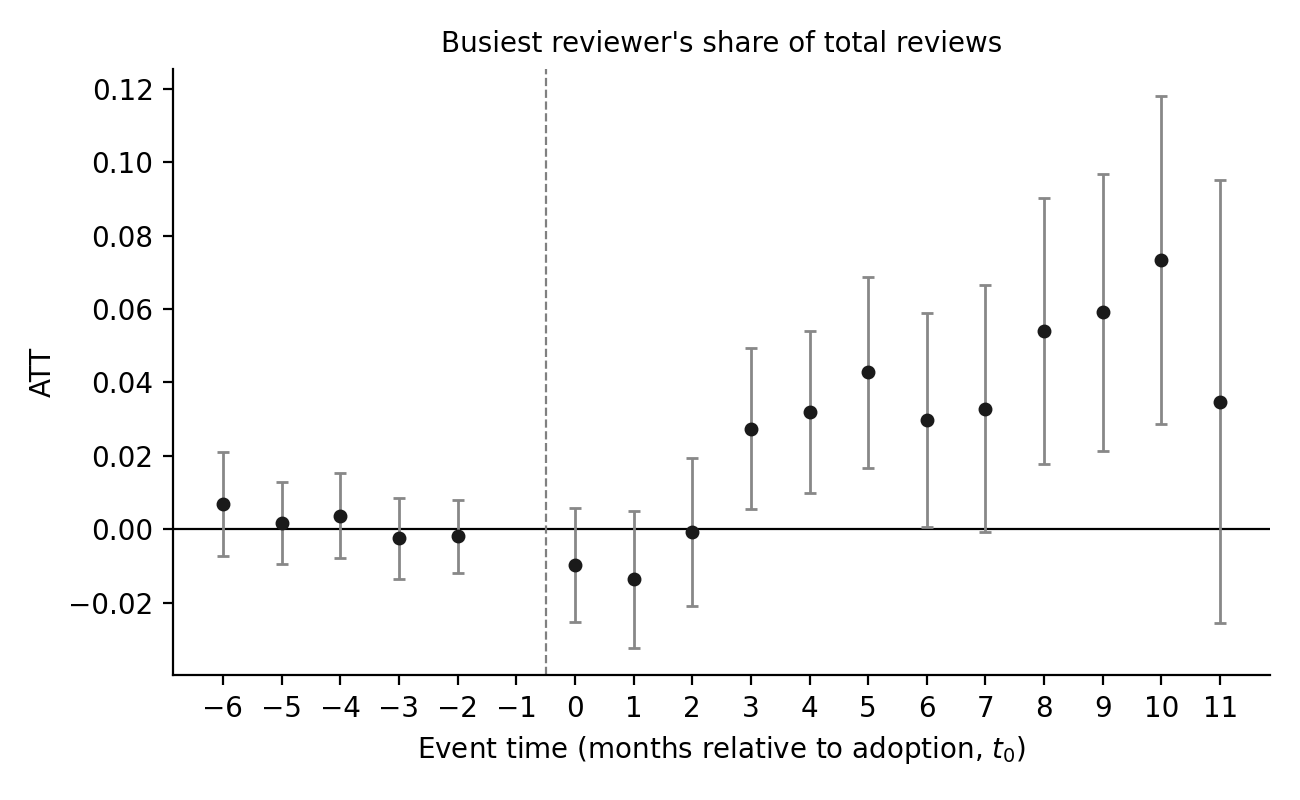
\includegraphics[width=0.48\textwidth]{figures/eventstudy_top1_share.png}
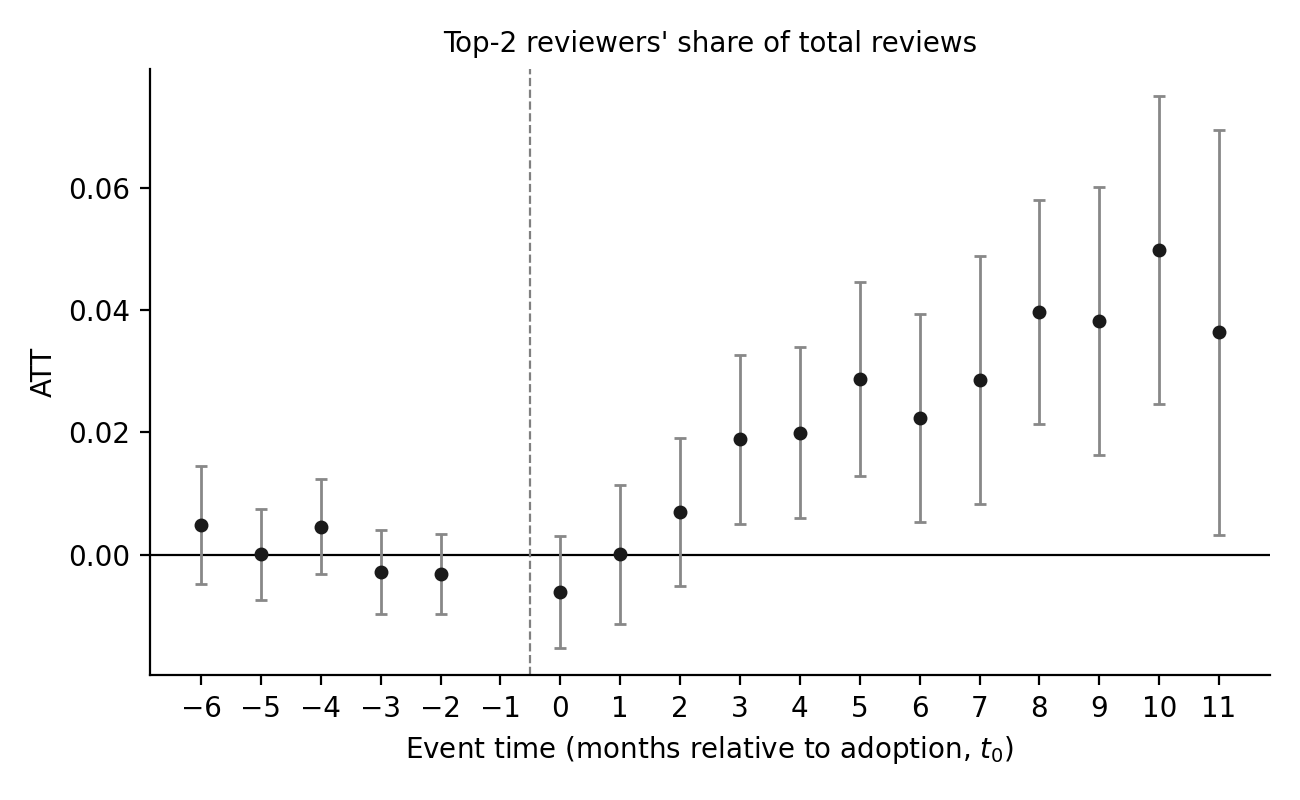
\includegraphics[width=0.48\textwidth]{figures/eventstudy_top2_share.png}
\caption{Event-study coefficients for top-1 (left) and top-2 (right)
reviewer share of total review activity. Dashed line marks the last
pre-period lead before adoption; error bars are 95\% CIs.}
\label{fig:top_share}
\end{figure}

The top-2 share result is consistent with three different mechanisms
that a share measure alone cannot separate: the core reviewer's own
absolute review volume could be rising (\emph{core absorbs}), reviewers
outside the core could be doing less even while the core's own volume
stays flat (\emph{periphery withdraws}), or new reviewers could simply
stop joining, shrinking the pool without any existing reviewer changing
behavior (\emph{entry stops}). One decomposition worth stating precisely
because it is easy to over-read: on the same share scale,
\texttt{second\_only\_share} (the rank-2 reviewer's share alone) is flat
($-0.002$, $p=0.66$) and \texttt{tail\_share} (everyone outside the top
two) falls by exactly as much as top-2 share rises ($-0.015$,
$p<0.001$). This is not a second, independent confirmation of
peripheral withdrawal: because \texttt{tail\_share} is defined as
$1-\text{top2\_share}$ for every observation, its estimate is an exact
arithmetic mirror of the top-2 share result already reported, not new
evidence. What the decomposition legitimately adds is narrower: the
offsetting movement is not concentrated in the rank-2 reviewer
specifically, consistent with a single core reviewer gaining share
rather than a two-person team expanding. Adjudicating between the three
mechanisms above requires an absolute-count measure that a share cannot
provide by construction; Section 7 reports our progress toward exactly
that test.

\subsection{H2 -- Review latency: faster turnaround, with a caveat}

Time-to-first-review falls by 65 hours on average (pre-trend $p=0.59$)
and time-to-merge falls by 63 hours (pre-trend $p=0.90$); both remain
significant under the bootstrap-corrected SE ($p=0.025$ and $p=0.021$
respectively, weaker than the analytic-SE readings of $p=0.002$ and
$p=0.009$ but still below conventional thresholds). Both are sign-stable
across every caliper we tested, and
Figure~\ref{fig:latency} shows the effect present from adoption onward.
On caliper stability and pre-trend cleanliness alone these would be our
strongest estimates. However, the mean-reversion diagnostic finds treated
repositories reverting from extreme pre-period latency somewhat more
sharply than controls---an asymmetry not present for concentration or
iteration---most pronounced for time-to-merge on the raw-hours scale
(slope $-0.90$ treated vs.\ $-0.60$ control). Because duration data are
heavily right-skewed (Table~\ref{tab:descriptives}), we re-ran the
diagnostic on $\log(1+\text{hours})$: the gap shrinks substantially (to
$-0.63$ vs.\ $-0.54$, roughly a 17\% gap, and a 13\% gap for
time-to-first-review), indicating most, though not all, of the raw-scale
asymmetry is a mechanical artifact of skew. We report these two estimates
as real but somewhat less secure than the concentration and iteration
estimates.

\begin{figure}[htbp]
\centering
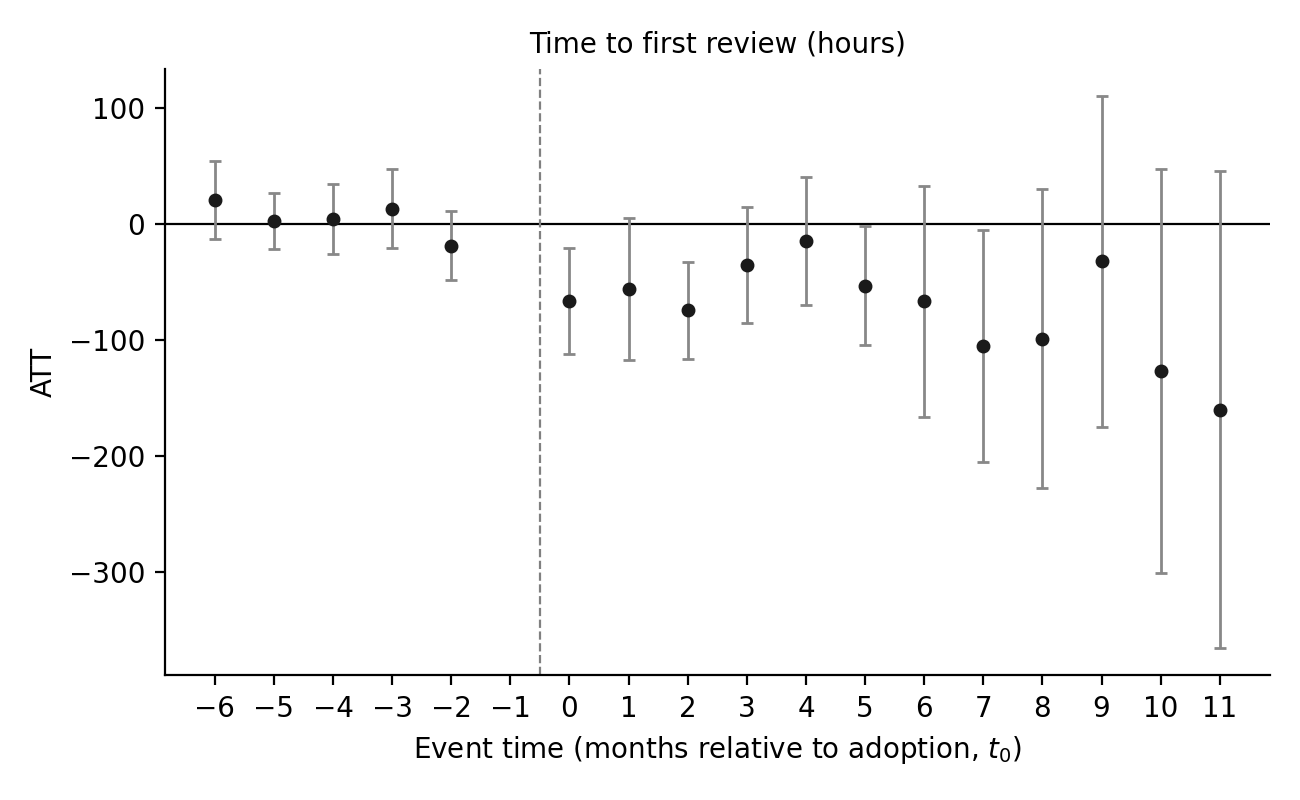
\includegraphics[width=0.48\textwidth]{figures/eventstudy_time_to_first_review_hours.png}
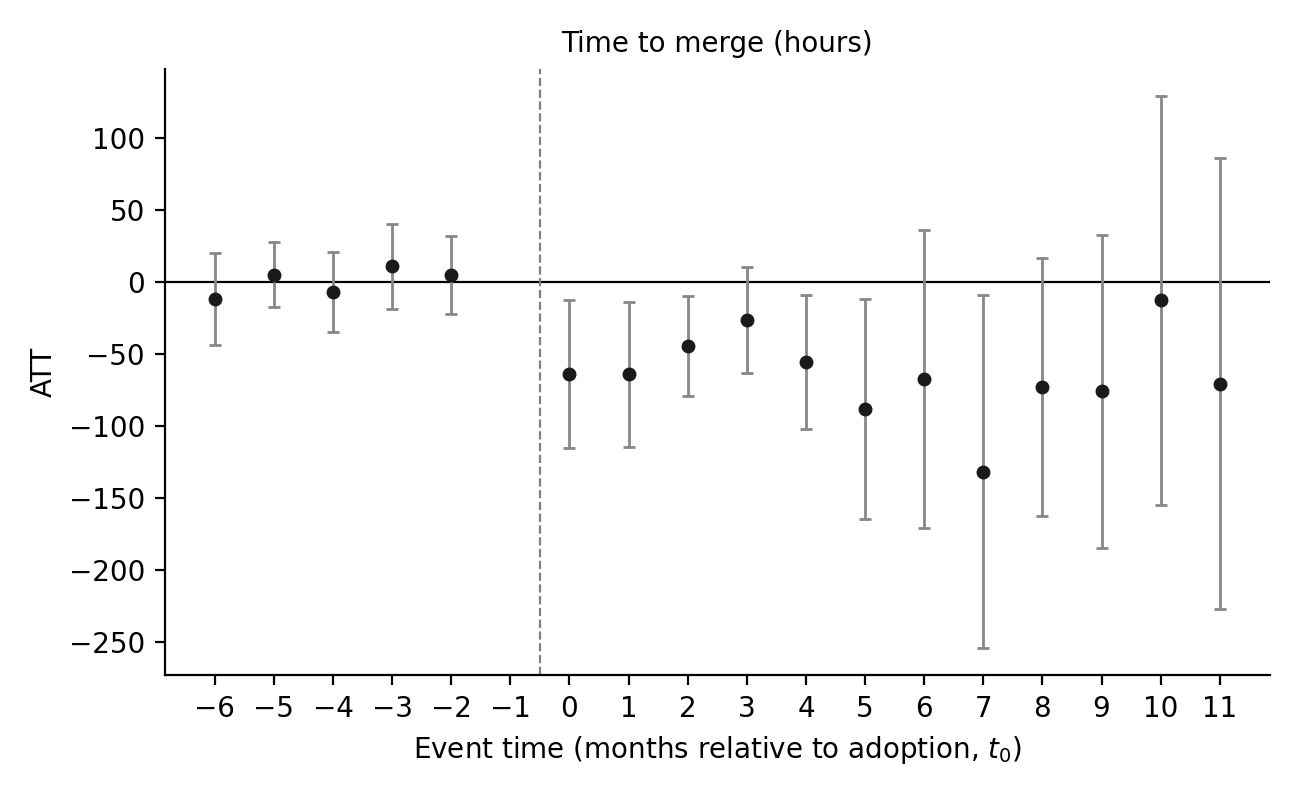
\includegraphics[width=0.48\textwidth]{figures/eventstudy_time_to_merge_hours.png}
\caption{Event-study coefficients for time to first review (left) and time
to merge (right), in hours.}
\label{fig:latency}
\end{figure}

\subsection{H3 -- Review iteration: more rounds per pull request}

Review rounds per merged PR increase by 0.18 on average (pre-trend
$p=0.19$), significant under both the analytic SE ($p<0.001$) and the
bootstrap-corrected SE ($p=0.027$), sign-stable at four of the five
calipers tested (the pre-trend fails only at caliper 0.35).
Figure~\ref{fig:rounds} shows the effect concentrated in the first six
post-adoption months. The mean-reversion diagnostic shows treated
repositories reverting \emph{less} than controls ($-0.31$ vs.\ $-0.52$),
again the opposite of a selection concern.

\begin{figure}[htbp]
\centering
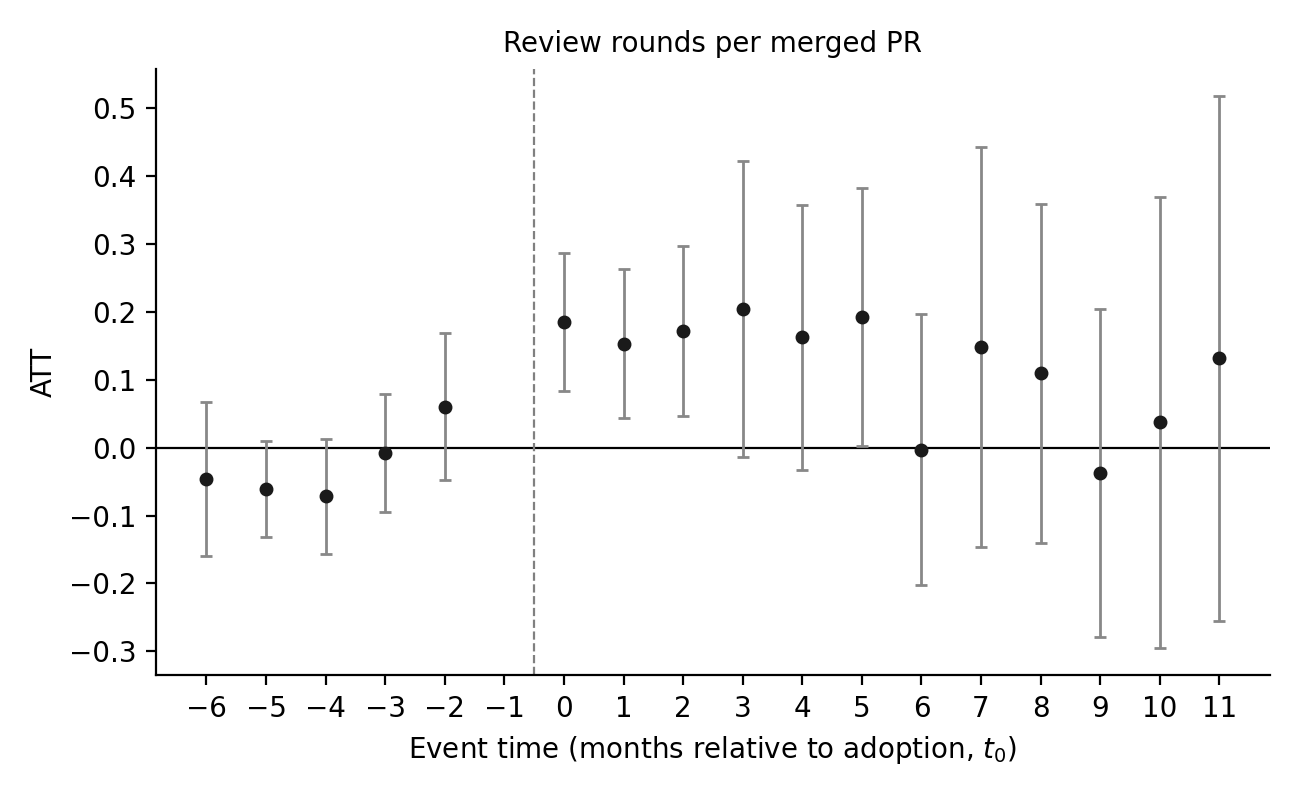
\includegraphics[width=0.6\textwidth]{figures/eventstudy_review_rounds.png}
\caption{Event-study coefficients for review rounds per merged PR.}
\label{fig:rounds}
\end{figure}

\subsection{Does the adoption mode matter?}
\label{sec:signal-type}

The verification-cost account in Section 2.1 does not obviously predict
whether concentration should differ between repositories where an
autonomous agent authors pull requests directly versus repositories where
a human commits with AI assistance but remains the nominal author. We
test this by splitting treated/control pairs on the treated repository's
adoption-signal composition (Section 3.2): ``agent'' repositories (an
autonomous-authorship signal fired, $n=1{,}383$ pairs) versus
``assisted'' repositories (only a co-authorship-trailer signal fired,
$n=388$ pairs), each re-estimated with its own subsample-specific
bootstrap SE and compared with a formal difference test rather than two
separate significance tests. Table~\ref{tab:signaltype} reports the
result.

\begin{table}[htbp]
\centering
\caption{Signal-type sensitivity: agent-authored vs.\ human-assisted adopters}
\label{tab:signaltype}
\small
\begin{tabular}{lrrl}
\toprule
Outcome & Agent ATT & Assisted ATT & Difference ($p$) \\
\midrule
Top-1 review share       & $+0.010$ (n.s.)   & $+0.039^{*}$   & $0.114$ (n.s.) \\
Top-2 review share       & $+0.009$ (n.s.)   & $+0.033^{***}$ & $0.037^{*}$ \\
Time to first review (h) & $-57.3$ (n.s.)    & $-73.6^{*}$    & $0.755$ (n.s.) \\
Time to merge (h)        & $-67.2^{*}$       & $-43.4$ (n.s.) & $0.601$ (n.s.) \\
Review rounds/PR         & $+0.24^{*}$       & $-0.01$ (n.s.) & $0.096$ (n.s.) \\
\bottomrule
\end{tabular}
\caption*{\footnotesize All entries use subsample-specific
bootstrap-corrected SEs. Difference $p$ from a two-sample $z$-test on
independent bootstrap SEs. $^{*}p<0.05$, $^{***}p<0.001$.}
\end{table}

Only the top-2-share difference survives correction ($p=0.037$):
concentration is larger for assisted adopters than for agent adopters.
The point-estimate gap for top-1 share and for review rounds points the
same direction but is not statistically confirmed once properly
bootstrapped---a naive reading of the (weaker) analytic SEs would have
over-claimed an agent-specific iteration effect that we do not, in fact,
find to be statistically distinguishable from the assisted-adopter
estimate. We treat ``adoption mode moderates concentration'' as
suggestive rather than established, resting on a single outcome among
five tested, and we do not carry an adoption-mode-specific iteration
claim forward. Latency shows no significant difference by adoption mode
in either direction.

\subsection{Does the pre-existing reviewer pool matter?}
\label{sec:heterogeneity}

We also test whether a repository's pre-existing reviewer-pool size
moderates H2 or H3, splitting pairs at the median of the treated
repository's own pre-period mean reviewers per PR (a genuinely
pre-treatment, behavioral measure, distinct from the structural,
snapshot-based covariates used for matching), and again using a formal
between-group difference test on bootstrap-corrected SEs rather than
comparing two separate significance tests. Table~\ref{tab:heterogeneity}
reports the result.

\begin{table}[htbp]
\centering
\caption{Reviewer-pool heterogeneity: small vs.\ large pre-existing pool}
\label{tab:heterogeneity}
\small
\begin{tabular}{lrrl}
\toprule
Outcome & Small-pool ATT & Large-pool ATT & Difference ($p$) \\
\midrule
Time to first review (h) & $-53.2$ (n.s.)$^{\dagger}$ & $-80.0$ (n.s.) & $0.650$ (n.s.) \\
Time to merge (h)        & $-64.8^{*}$                & $-56.7$ (n.s.) & $0.885$ (n.s.) \\
Review rounds/PR         & $+0.28^{**}$$^{\dagger}$    & $+0.08$ (n.s.) & $0.276$ (n.s.) \\
\bottomrule
\end{tabular}
\caption*{\footnotesize $^{\dagger}$Fails its own joint pre-trend test in
this subsample. $^{*}p<0.05$, $^{**}p<0.01$.}
\end{table}

No outcome shows a statistically confirmed difference by pre-existing
reviewer-pool size once tested properly. This is a case where correcting
inference reverses a conclusion we would otherwise have drawn: the
review-rounds split looks significant on the analytic SE ($p=0.032$,
suggesting iteration concentrates in small-pool repositories), but the
bootstrap-corrected difference test gives $p=0.276$, and the driving
small-pool estimate independently fails its own pre-trend test regardless.
We find no evidence that the pre-existing reviewer pool moderates either
the latency or the iteration response to adoption.

\subsection{Sensitivity to parallel-trend violations}
\label{sec:trend-sensitivity}

The joint pre-trend test used throughout is a binary pass/fail check.
To assess how much an undetected violation could plausibly explain
away a given estimate, we fit a weighted linear trend through each
outcome's five pre-period lead coefficients, extrapolate it forward to
the average post-period horizon, and compute the breakdown
slope---the per-month drift that would need to hold for the extrapolated
trend to fully explain the observed pooled ATT---expressed as a multiple
of the actually-estimated pre-trend slope's own standard error.
Table~\ref{tab:breakdown} reports the result for all five outcomes
supporting H1--H3.

\begin{table}[htbp]
\centering
\caption{Parallel-trend sensitivity: breakdown slope in units of the estimated pre-trend's SE}
\label{tab:breakdown}
\small
\begin{tabular}{lr}
\toprule
Outcome & Breakdown slope \\
\midrule
Top-1 review share       & 2.6$\times$ (wrong-signed pre-trend---strengthens the estimate) \\
Top-2 review share       & 3.4$\times$ (wrong-signed pre-trend---strengthens the estimate) \\
Time to first review (h) & 3.7$\times$ (same-signed---extrapolation erodes $\sim$36\% of the ATT) \\
Time to merge (h)        & 3.8$\times$ \\
Review rounds/PR         & 3.0$\times$ (same-signed---extrapolation erodes $\sim$55\% of the ATT) \\
\bottomrule
\end{tabular}
\end{table}

The concentration estimates are the most robust to an undetected
violation: their actual pre-period leads run in the \emph{opposite}
direction from the post-period effect, so extrapolating them forward
would make the estimated effect larger, not smaller. The latency and
iteration estimates have same-signed pre-leads that, extrapolated, would
erode 36--55\% of the raw ATT---not enough to change the sign or
significance of either estimate, but consistent with holding H2 and H3 to
the more cautious evidentiary standard we apply throughout.

\subsection{Robustness at a glance}

The detailed caliper and mean-reversion figures above are dispersed
across three subsections; Table~\ref{tab:robustness} collects them in one
place for the five outcomes that support H1--H3 (the review-intensity
outcomes and the raw top-1 review count are excluded here because they do
not pass the identification checks described in Sections 5.1--5.2 and are
not carried forward as findings).

\begin{table}[htbp]
\centering
\caption{Robustness summary for the outcomes supporting H1--H3}
\label{tab:robustness}
\small
\begin{tabular}{lll}
\toprule
Outcome & Caliper stability (5 tested) & Mean-reversion \\
\midrule
Top-1 review share (H1)   & Stable, all 5 calipers        & No concern \\
Top-2 review share (H1)   & Stable, all 5$^{\dagger}$      & No concern \\
Time to first review (H2) & Stable, all 5 calipers        & Mild caveat \\
Time to merge (H2)        & Stable, all 5 calipers        & Caveat (asymmetry) \\
Review rounds (H3)        & Stable 5/5, sig.\ 4/5$^{\dagger}$ & No concern \\
\bottomrule
\end{tabular}
\caption*{\footnotesize $^{\dagger}$Joint pre-trend test fails at one of
the five calipers tested (0.35 SD); the estimate's sign does not change at
any caliper. ``Mean-reversion'' summarizes the diagnostic in the relevant
subsection above; ``mild caveat'' and ``caveat (asymmetry)'' refer to the
same treated/control gap discussed for H2, shown there on both the raw
and log scale.}
\end{table}

The cluster-robust SE used throughout is a documented approximation, not
the fully rigorous BJS variance estimator (Section 4.2). We validate it
with a 300-replicate repo-pair cluster bootstrap---resampling matched
pairs with replacement and refitting the full two-way FE model on each
resample, with a uniquified entity identifier per replicate so that a
pair drawn twice contributes two independent pseudo-clusters rather than
being folded into one entity's average. Table~\ref{tab:bootstrap}
compares the resulting bootstrap SE against the analytic SE for all five
outcomes supporting H1--H3.

\begin{table}[htbp]
\centering
\caption{Analytic vs.\ bootstrap-corrected standard errors}
\label{tab:bootstrap}
\small
\begin{tabular}{lrrrr}
\toprule
Outcome & Analytic SE & Bootstrap SE & Ratio & Corrected $p$ \\
\midrule
Top-1 review share       & 0.0064 & 0.0089 & 1.39$\times$ & 0.052 \\
Top-2 review share       & 0.0034 & 0.0050 & 1.45$\times$ & 0.003 \\
Time to first review (h) & 21.40  & 28.91  & 1.35$\times$ & 0.025 \\
Time to merge (h)        & 24.18  & 27.10  & 1.12$\times$ & 0.021 \\
Review rounds/PR         & 0.045  & 0.082  & 1.83$\times$ & 0.027 \\
\bottomrule
\end{tabular}
\end{table}

The analytic SE understates true uncertainty by 12--83\% across these
five outcomes. Every outcome remains significant at $p<0.05$ under the
corrected SE except top-1 review share, which drops from comfortably
significant to borderline ($p=0.052$)---which is why we treat top-2
share, not top-1 share, as the more secure carrier of the concentration
finding throughout this paper (Section 5.2). All reported $t$-statistics
and $p$-values for the five H1--H3-supporting outcomes, including in
Table~\ref{tab:main} and in Sections 5.5--5.6 above, use this corrected
SE, not the analytic one.

\subsection{Summary of the DiD report}

Across eight outcomes, three difference-in-differences estimates hold up
under the full validation sequence, now including bootstrap-corrected
inference---review-share concentration (two measures, though top-2 share
is the more secure of the two), review latency (two measures, with a
noted caveat), and review iteration---while review intensity shows no
reliable effect and one concentration measure (the raw count) is excluded
on identification grounds. The two exploratory splits we additionally
tested are largely null once corrected: adoption mode moderates only
top-2 share, and the pre-existing reviewer pool moderates neither latency
nor iteration. This pattern of estimates that survive a deliberately
adversarial validation sequence---not any single estimate, and not the
splits that failed to survive it---is the paper's empirical contribution.

\section{Discussion: What These Estimates Suggest}

The estimates in Table~\ref{tab:main} do not support a story in which AI
coding assistance simply reduces the total volume of human oversight
applied to code (the review-intensity benchmark is null). They support
H1--H3, consistent with the verification-cost account developed in
Section 2.1: review work does not disappear, but comes to depend on
fewer specialists (H1), is processed faster once specialized (H2), and
is calibrated through more, cheaper verification touchpoints rather than
one gate (H3). We revisit each below in light of what Section 5's
robustness battery adds beyond the headline estimate.

\textbf{H1 -- Dependence.} The finding is more precisely a top-2, not a
top-1, phenomenon: under corrected inference, the core reviewer's own
share is only borderline significant, while the top-two reviewers'
combined share is robust. This is worth taking seriously rather than
rounding away---it suggests the specialization Section 2.1 predicts may
form around a small team of two, not a single irreplaceable gatekeeper, a
distinction with direct single-point-of-failure implications discussed
below. The signal-type split (Section 5.5) adds that this dependence
is significantly larger for human-directed, AI-assisted adopters than for
autonomous-agent adopters (top-2 share difference $p=0.037$)---plausibly
because a human co-author retains some review-worthy context an
autonomous agent's PR does not, which may itself route review toward
whoever already understands that context, i.e., the same verification-cost
mechanism operating with a different reviewer-side starting point.
Section 5.2's mechanism decomposition on the share scale (core's
second-place partner flat, tail share falling) is arithmetic, not
independent evidence, once the top-2 share result is known---it tells us
\emph{where within the non-core group} the offsetting movement falls,
not whether the core reviewer's own absolute workload rose. That
question is separate, and is what the fixed-identity extraction
(Section 7) is designed to answer directly; our own preliminary read on
a partial sample leans toward the core reviewer's own count being flat
or falling, which would describe consolidation through the periphery's
retreat rather than the core taking on more work---the opposite of a
straightforward reading of ``the core reviewer works harder.''

\textbf{H2 -- Acceleration.} Review latency falls, and does so consistently
regardless of adoption mode or pre-existing reviewer-pool size (Sections
5.5--5.6): the effect is general, not concentrated in a particular kind of
repository. We hold H2 to the most cautious standard of the three
findings, however, because the mean-reversion diagnostic (Section 4.3)
finds a modest, only partially scale-driven treated/control asymmetry not
present for H1 or H3---some part of the observed speed-up may reflect
regression from an unusually slow pre-period baseline rather than a pure
treatment effect, even though the parallel-trend breakdown analysis
(Section 5.7) shows the estimate would survive a moderately large
undetected violation.

\textbf{H3 -- Iteration.} Faster review does not mean lighter-touch review:
rounds per pull request rise. This combination---faster, narrower, more
iterative review---is difficult to explain with a single-mechanism theory
of either automation-induced complacency or automation-induced distrust,
and complicates a straightforward reading of human--AI augmentation
theory: augmentation here does not show up as ``the same process, less
human effort,'' but as a restructured process with a different
distribution of who does the work and how quickly.

For engineering leaders, the dependence estimate is a single-point-of-
failure and lost-redundancy risk that will not show up in naive metrics
like PRs reviewed per team per week---this risk holds independent of
whether the concentrated reviewer's own workload rises, since fewer
people can approve a change either way, and the top-2, not top-1,
finding suggests the relevant risk unit may already be a two-person team
rather than one individual, worth monitoring as such directly; the
latency estimate should not be read, in isolation, as evidence that AI
adoption speeds up review for the whole team rather than for a shrinking
set of active reviewers; and the iteration estimate suggests that faster
review is being achieved through more frequent, not fewer, touchpoints.

\section{Limitations}

Our design shares limitations common to public-repository studies of AI
adoption. First, our adoption signal has an \textbf{attribution ceiling}:
it captures only \emph{visible} AI usage, biasing every reported ATT
toward zero and making it a lower bound rather than a population
estimate. Second, \textbf{selection into treatment} is not supported by
our mean-reversion diagnostic for the concentration or iteration
estimates, but a modest, partly scale-driven asymmetry remains for the
latency estimates even after a log transformation, which is why we report
those two estimates with a caveat rather than as unconditionally causal.
Third, our sample is drawn from public, sufficiently active,
sufficiently starred GitHub repositories stratified by language and
creation cohort; it is not a random sample of all software development
and may not generalize to closed-source or enterprise settings---though
\citet{he2026aiwrites}'s independent finding of roughly doubled
per-reviewer load at an enterprise adopting AI coding tools at scale is
at least directionally consistent with our concentration result in a very
different population, which we read as modest cross-context
corroboration rather than proof of generalizability. Fourth, our
standard errors are a cluster-robust approximation rather than the fully
rigorous BJS variance estimator; we validate, rather than merely
disclose, this approximation with a 300-replicate cluster bootstrap
(Section 5.8), which shows it understates true uncertainty by 12--83\%,
and we report the corrected inference throughout---but the bootstrap
itself still relies on the same diagonal-covariance-style approximation
the analytic SE does, not a full re-derivation of the BJS variance
estimator. Fifth, the multiple comparisons in this paper extend beyond
the original eight-outcome family: the signal-type and reviewer-pool
splits in Sections 5.5--5.6 add ten further estimates and their
difference tests. We treat these splits as exploratory rather than
confirmatory throughout, which is a substantively different (and more
conservative) claim than applying a single family-wise correction across
everything; a reader who prefers the latter should treat the $p=0.037$
top-2-share signal-type difference, in particular, as more fragile than
it appears in isolation. Sixth, our central concentration measure
(top-2 review share) identifies \emph{how much} of review activity goes
to a repository's core reviewers but not \emph{who} they are over
time; we cannot yet confirm from the data reported here whether the same
individual(s) hold that position across a repository's adoption window,
which is necessary to fully support the bus-factor interpretation offered
in Section 6---this verification is in progress on a reviewer-identity
extension of this dataset and is not yet complete as of this draft.
Finally, this design measures a lower bound on review-process change
attributable to \emph{detectably} AI-assisted work and cannot speak to
the (likely substantial) share of AI-assisted contributions our signal
does not detect.

\section{Conclusion}

Grounded in a verification-cost account of human--AI collaboration and
estimated on 1,771 matched GitHub repository pairs and 20,188
repository-months of review-process data, we find that a repository's
adoption of an AI coding tool does not detectably change how many people
review its pull requests, but does concentrate review activity on its
top two reviewers specifically (H1), shorten review latency (H2), and
increase the number of review rounds per pull request (H3)---a pattern
validated against pre-trend testing, five-caliper matching sensitivity, a
balanced-panel restriction, a mean-reversion diagnostic, a parallel-trend
breakdown-sensitivity analysis, a 300-replicate cluster bootstrap that
corrects for a meaningfully understated analytic standard error, and a
re-verification of the adoption signal itself. Splitting adopters by
signal type further shows that concentration is significantly larger for
human-directed, AI-assisted adopters than for autonomous-agent adopters,
while a repository's pre-existing reviewer-pool size moderates neither
the latency nor the iteration response once tested with a proper
between-group difference test---a conclusion that itself required
correcting a naive analytic-SE result that had suggested otherwise. This
pattern suggests that the organizational adjustment to AI-assisted coding
is better described as concentrating oversight onto fewer reviewers than
as a simple reduction or expansion of oversight, and
it points toward gatekeeping \cite{allen1977gatekeepers},
expertise-specialization, and
iterative-trust-calibration as the theoretical mechanisms most worth
testing directly in future work. Three extensions follow directly from
what this paper leaves open: confirming, with reviewer-identity data
currently being collected, that the same individuals persist in the
concentrated reviewer role across a repository's adoption window, rather
than the aggregate share statistic reflecting a rotating cast; an
instrument for adoption timing or a triple-differences design targeting
the residual latency-estimate caveat we identify here; and a fixed-window,
competing-risk treatment of unmerged and still-open pull requests, which
our merged-PR-only latency measure cannot itself rule out as a source of
sample-composition bias.

\bibliographystyle{plainnat}
\bibliography{references}
% NOTE: entries pulled from references.bib (shared with slides.tex). Some
% entries carry a `note` field flagging incomplete bibliographic detail --
% verify against the original sources before submission.

\end{document}
